\setlength{\columnsep}{3pt}
\begin{flushleft}
	\bigskip
	\begin{figure}[h!]
	\centering
	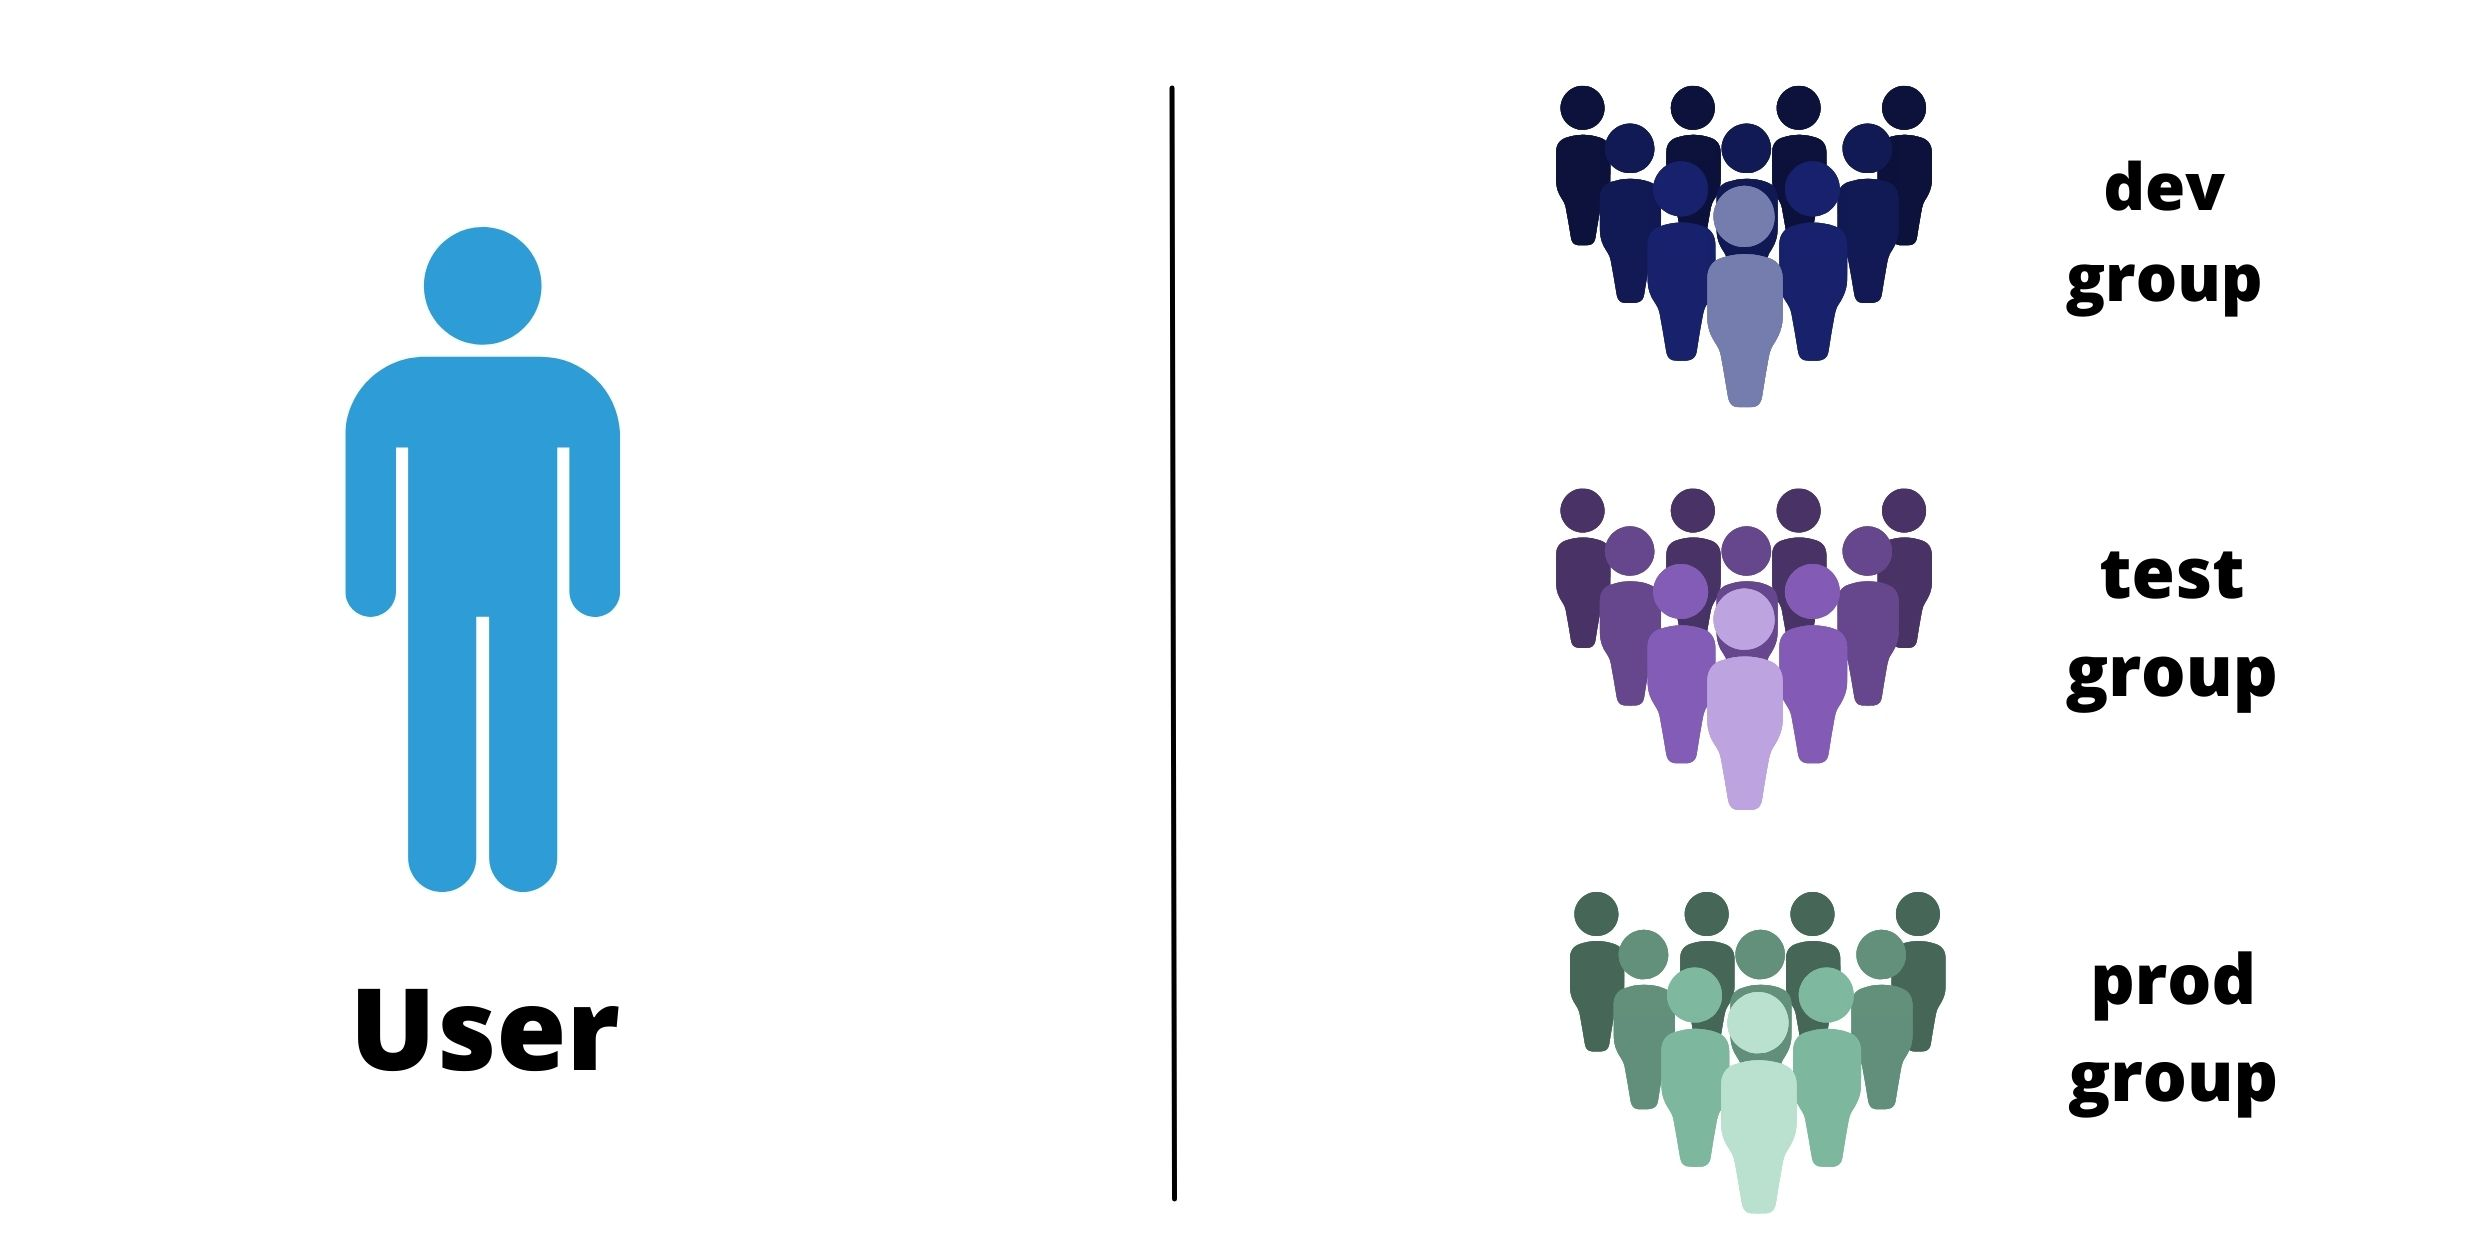
\includegraphics[scale=.2]{content/chapter4/images/user_group.jpg}
	\caption{User V/S Group}
	\label{fig:user_group}
	\end{figure}
	\bigskip

	\begin{itemize}
		\item Group is a collection of users.
		\item Users are grouped together for granting common permissions to all members of a group.
		\item A user can be a member of more than one group.
	\end{itemize}

\newpage
	\paragraph{Types of group}
	
	\begin{itemize}
		\item \textbf{Primary group}:
		\begin{itemize}
			\item Primary group are automatically generated while creating a user.
			\item A user becomes member of their primary group automatically.
			\item Primary group have same name as the username \& a unique group ID.
			\item \textbf{One user can have one and only one primary group}.
		\end{itemize} 
		\item \textbf{Secondary or supplementary group}:
		\begin{itemize}
			\item Secondary group are created separately with the help of \textbf{groupadd} command.
			\item Multiple users can be added to the secondary group.
			\item \textbf{One user can have more than one secondary groups}.
		\end{itemize} 
	\end{itemize}
	
	\begin{figure}[h!]
		\centering
		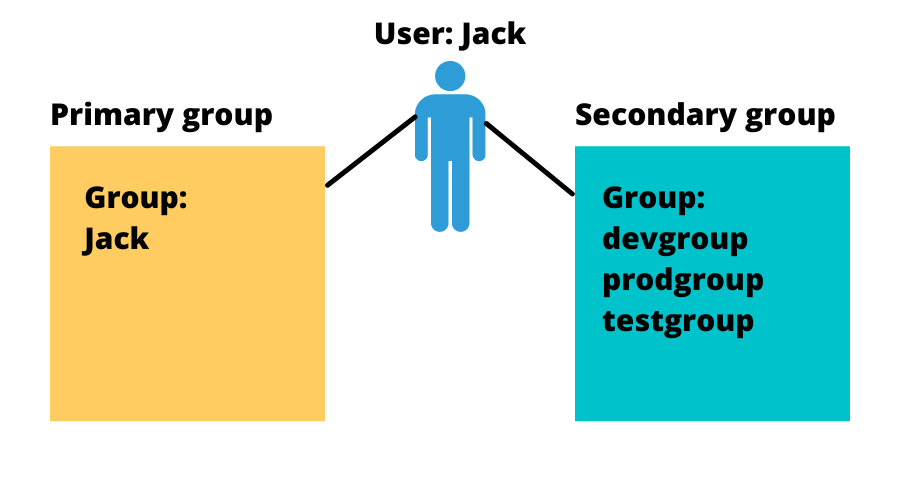
\includegraphics[scale=0.5]{content/chapter4/images/type_group.png}
		\caption{Primary and Secondary group}
		\label{fig:prime_secondary_group}
	\end{figure}
	


\end{flushleft}

\newpage

